\section{Funktionsweise}

\begin{frame}{Begriffe}
  \begin{Definition}
    Ein \textbf{Repository} ist ein verwaltetes Verzeichnis zur Speicherung und Beschreibung von digitalen Objekten für ein digitales Archiv.\cite{WREP}
  \end{Definition}

  \begin{Definition}
    \textbf{Remote origin} ist ein Verweis auf das \textit{remote} Repository (also eine URL).
  \end{Definition}

  \note[item]{Bei uns: ein Repository enthält Programmpakete und zugehörige Metadaten}
  \note[item]{Bei uns: Logs, temporäre Dateien oder Nutzerspezifische Config-Dateien werden nur lokal gespeichert!}
\end{frame}

\begin{frame}[fragile]{.git Ordner}
  \begin{itemize}
    \item Alle \textbf{git-Daten} liegen im .git Repository mit optionalen Ausnahmen
  \end{itemize}
  \pause
  \begin{lstlisting}[basicstyle=\tiny]
  $ ls -l .git
  total 40
  -rw-r--r--   1 joeldierkes  staff   15 Mar 29 21:43 COMMIT_EDITMSG
  -rw-r--r--   1 joeldierkes  staff   23 Mar 29 21:43 HEAD
  -rw-r--r--   1 joeldierkes  staff  137 Mar 29 21:43 config
  -rw-r--r--   1 joeldierkes  staff   73 Mar 29 21:43 description
  drwxr-xr-x  13 joeldierkes  staff  416 Mar 29 21:43 hooks
  -rw-r--r--   1 joeldierkes  staff  209 Mar 29 21:43 index
  drwxr-xr-x   3 joeldierkes  staff   96 Mar 29 21:43 info
  drwxr-xr-x   4 joeldierkes  staff  128 Mar 29 21:43 logs
  drwxr-xr-x  10 joeldierkes  staff  320 Mar 29 21:43 objects
  drwxr-xr-x   4 joeldierkes  staff  128 Mar 29 21:43 refs
  \end{lstlisting}

  \note[item]{Der .git Ordner kann auch durch das Umbenennen der Umgebungsvariable \textbf{GIT\_DIR} anders benannt werden}
  \note[item]{Git guckt im aktuellen Verzeichnis ob der .git Ordner gefunden wurde, falls nicht wird dies rekursiv für alle Parent-Directories gemacht}
\end{frame}

\begin{frame}{Blob}
  \begin{Definition}
    Ein \textbf{Blob} (\glqq \textit{binary large object} \grqq ) ist eine Version einer Datei.
  \end{Definition}
  \begin{itemize}
    \pause
    \item Enthält den Inhalt einer Datei, aber nicht deren Metadaten (Dateiname, Erstelldatum, ...)
    \pause
    \item Ist eindeutig durch den SHA-1 Wert bestimmt (Kollision verschwindend gering)
  \end{itemize}

  \note[item]{Ein Blob wird \textbf{komprimiert} gespeichert}
  \note[item]{Die annahme, dass zwei Elemente mit gleichem Hash-Wert auch gleich sind, ist in diesem Fall ausreichend (genügend geringe Chance für eine Kollision)}
\end{frame}

\begin{frame}{Tree}
  \begin{Definition}
    Ein \textbf{Tree} enthält Informationen eines Systemordners.
  \end{Definition}
  \begin{itemize}
    \pause
    \item Verweist auf Blobs und weitere (Sub-)Trees
    \pause
    \item Enthält auch Daten wie Datei- und Pfadnamen von Blobs und Trees
    \pause
    \item Ist ebenfalls eindeutig durch den SHA-1 Wert bestimmt
  \end{itemize}

  \note[item]{Bildet das Dateisystem in git ab, allerdings über verschiedene Versionen hinweg}
\end{frame}

\begin{frame}{Commit}
  \begin{Definition}
    Ein \textbf{Commit} enthält Informationen zu einer Änderung des Repositories.
  \end{Definition}
  \begin{itemize}
    \pause
    \item Verweist auf einen Tree und einen oder mehrere \glqq Parent\grqq{} Commits
    \pause
    \item Änthält Informationen zu Autor, Datum und weiteres
    \pause
    \item Hat einen semantischen Sinnzusamenhang
    \pause
    \item Ist ebenfalls eindeutig durch den SHA-1 Wert bestimmt
  \end{itemize}

  \note[item]{Im Repository kann nur zwischen Commits gewechselt werden, ein Zwischenzustand ist nicht möglich}
  \note[item]{kann Kommentiert werden, sollte sinnvoll kommentiert sein}
\end{frame}

\begin{frame}{Commit}
  \href{https://medium.com/@gohberg/the-biggest-misconception-about-git-b2f87d97ed52}{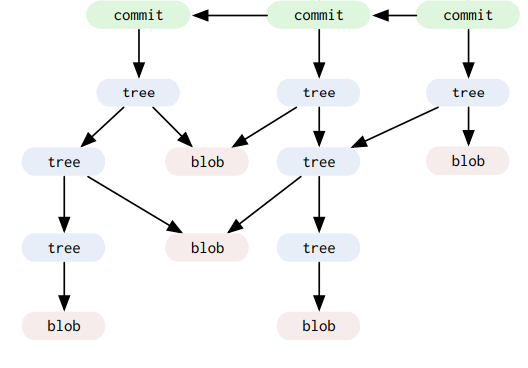
\includegraphics[scale=0.5]{./section/pictures/internes.png}}

  \note[item]{Ein Graph, der mehere Blobs, Trees und Commits zeigt}
  \note[item]{Im Späteren werden Blobs und Trees nicht mehr gezeigt $\rightarrow$ Commit Graph}
\end{frame}

\begin{frame}{Tags}
  \begin{Definition}
    Ein \textbf{Tag} referenziert auf ein Objekt, meistens ein Commit.
  \end{Definition}
  \begin{itemize}
    \pause
    \item Sollte einen sinnvollen Namen besitzen
  \end{itemize}

  \note[item]{Eine Möglichkeit, einen Commit zu benennen und ihn so leichter zu finden}
  \note[item]{Meist für Auslieferungen o.ä.}
\end{frame}

\begin{frame}{Index}
  \begin{itemize}
    \item Temporäres Speichern von Blobs und Trees, bis diese Commitet werden
    \pause
    \item Damit sind die Änderungen nicht zwingend im RRepository
    \pause
    \item Low-level, darauf sollte nie gearbeitet werden
    \pause
    \href{https://hackernoon.com/understanding-git-index-4821a0765cf}{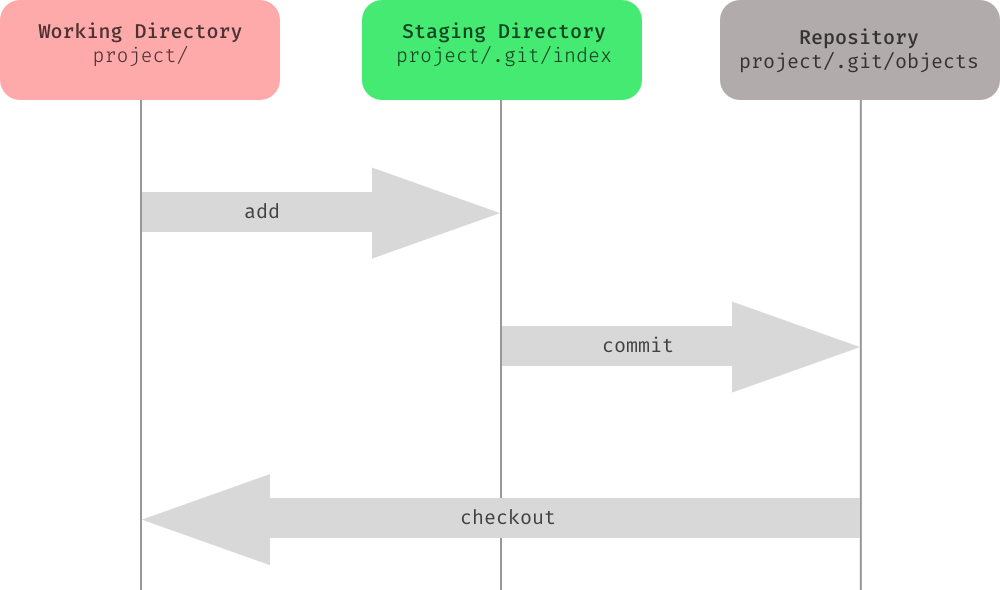
\includegraphics[scale=0.25]{./section/pictures/index.png}}
  \end{itemize}

  \note[item]{Arbeitsfluss:
    \begin{itemize}
      \item Im Working-Directory werden änderungen vorgenommen
      \item Im Stagin-Directory werden diese temporär gespeichert
      \item Im Repository werden diese dauerhaft und für alle commitet
    \end{itemize}}
  \note[item]{Dies sollte alles mit Befehlen/einem GUI umgesetzt werden, low-level sollte nichts verändert werden}
\end{frame}
